%%%%%%%%%%%%%%%%%%%%%%%%%%%%%%%%%%%%%%%%%%%%%%%%%%%%%%%%%%%%%%%%%%%%%%%%%%%%%%%%
% INTRODUCTION
\chapter{Introduction}
%%%%%%%%%%%%%%%%%%%%%%%%%%%%%%%%%%%%%%%%%%%%%%%%%%%%%%%%%%%%%%%%%%%%%%%%%%%%%%%%

File system metadata management is difficult to scale. The attention that the
topic has received, in both industry and academia, suggests that even decoupling
metadata IO from data IO so that these services can scale independently is
insufficient for today's workloads.  Cutting-edge techniques for scaling file
system metadata access are implemented in `clean-slate' file systems built from
the ground up, so users that want to leverage techniques from different file
systems must provision separate storage clusters. Adding software layers to the
compute stack in this way complicates system management because administrators
must now (1) configure data migrations across file system boundaries and (2)
compare file system metadata management techniques, which includes
understanding implementations and benchmarking systems with the workload.
Alternatively, developers can integrate multiple techniques into an existing
file system and expose configuration parameters to let users select metadata
management strategies. While this lets users compare techniques and minimizes
data movement, it further increases the size of the stack because software
layers are larger and their internals are more complex. This approach
complicates system management because if techniques do not match the workload
or a new technique becomes available, developers need to modify code, which
takes time and jeopardizes the robustness of the file system. 

% Problem: large systems are difficult to manage
%Systems that process and store large amounts of data (petabytes and beyond)
%are difficult to manage. 

The layering problem is getting worse because of the trends of modern
computing: data is too large, software is too complicated, hardware
characteristics are changing too fast, and events are too frequent. The
unmanageable nature of these hardware and software stacks is a result of
abstracting away complexity using layers. Black box abstraction has been a boon
to software because developers can focus on areas of their own expertise, but
three trends have broken this programming model and proliferated unmanageable
stacks:

\begin{itemize}
% Timeliness: layers on layers; {big stacks, overhead, proof}
\item \textbf{More Data}: The overwhelming volume, velocity, and veracity of today's
data shapes modern software. When data grows too large, we scale to larger
systems, either by scaling out or scaling up. Focusing on the scale-out model
has given birth to stacks, like Apache, that are used in industry,
laboratories, and academia. But the size of these stacks leads to increased
complexity, as code bases are larger and more
layered~\cite{sevilla:eurosys17-malacology}.

% Timeliness: extreme hetoregeneity {memory wall, more hardware, more runtimes}
\item \textbf{Extreme Heterogeneity}: Increased heterogeneity in software and
hardware requires large stacks just to manage resources.  Data centers are
larger and have faster devices because device and network speeds are scaling
much faster than DRAM speeds. The so-called memory
wall~\cite{wulf:sigarch1995-memory-wall} pushes resource management into
software runtimes, which must now manage large numbers of heterogeneous
devices. The increasing momentum behind disaggregated
storage~\cite{klimovic:asplos2017-reflex, klimovic:eurosys16-disagg}, a model
that uses software as the control plane and reduces the CPU requirements of
devices, is a result of prognoses that we are heading towards data centers that
need to provision a CPU per storage device~\cite{samuels:oss16}. Regardless of
where the future leads, the scale and complexity of software will continue to
scale with the size of the architectures they manage.

% Timeliness: oss faciliates transparency {vendor lock in, efficiency, collab}
\item \textbf{Open-source Sofware}: Open-source software is gaining traction because
it helps consumers avoid vendor lock in, it leads to more efficient
implementations, and it encourages collaboration. All these advantages are
rooted in transparency, as developers can work together to write code that
manages the extreme heterogeneity mentioned above, but it also lets developers
see the source code for the systems they use ``off-the-shelf". In short,
open-source software leads to more software because code can come from
different domains, organizations, and communities, and it is easier to write
optimizations for layers that are are fully exposed.

\end{itemize}

The stacks produced by these trends have longer code paths, duplicated
functionality, and lower performance.  The overhead of these stacks are so
high that many workloads can be outperformed by a single, scale-up node with
less resources~\cite{sevilla:discs2013-framework,
rowstron:hotcdp2012-hadoop-vs-single-node, schwarzkopf:hotcloud2012-7-sins,
gigaspaces:whitepaper2011-su-vs-so, michael:2007pdps-scale-up-x-scale-out}.  In
light of these trends, our solution is a concept called ``programmable
storage"~\cite{sevilla:eurosys17-malacology, watkins:hot17-declstor}.
Programmable storage facilitates the re-use and extension of existing storage
abstractions provided by the underlying software stack, to enable the creation
of new services via composition. This development process is faster than
reducing layers manually for new architectures with less
layers~\cite{bent:login16-hpc-trends} that may break backwards compatibility.
We add interfaces {\it into} a storage system's internal functionality to
facilitate application co-design, leading to more efficient implementations
that inherit the robustness of the underlying system with less code
duplication. This thesis uses the programmable storage approach to embed policy
engines into file system metadata substrates to control the behavior,
performance, and transparency of the entire software stack.

\section{Contributions}

This thesis argues that the programmable storage approach is the correct model
for scaling global namespaces and designing effective file system
metadata management policies. We design policies for three metadata management
techniques: subtree load balancing, subtree semantics, and subtree schemas.
The first two expand on a strong foundation of related work while the third is
a novel idea.

First, we present a methodology for programmable load balancing policies for
file system metadata.  To help decouple policy from mechanism, we introduce a
programmable storage system, Mantle, that lets the designer inject custom
balancing logic. We show the flexibility and transparency of this approach by
replicating the strategy of a state-of-the-art metadata balancer and conclude
by comparing this strategy to other custom balancers on the same system. We
also show how the data management language and policy engine from Mantle turns
out to be an effective control plane for managing ZLog sequencers and ParSplice
caches.

Second, we present a methodology for programmable consistency and durability in
a global namespace. Our prototype, Cudele, lets clients specify their
consistency/durability requirements and dynamically assign them to subtrees in
the same namespace, allowing users to optimize subtrees over time and space for
different workloads. We confirm the performance benefits of techniques
presented in related work but also explore new consistency/durability metadata
designs, all integrated over the same storage system. By custom fitting a
subtree to a create-heavy application, we we show performance improvements when
we custom fit subtree semantics to applications such as checkpoint-restart
(91.7\(\times\) speedup), user home directories (0.03 standard deviation from
optimal), and users checking for partial results (2\% overhead).

Third, we present a methodology for generating namespaces automatically and
lazily, without incurring the costs of traditional metadata management,
transfer, and materialization.  We introduce namespace generators and schemas
to describe file system metadata structure in a compact way. If clients and
servers can express the namespace in this way, they can compact metadata,
modify large namespaces more quickly, and generate only relevant parts of the
namespace. The result is less network traffic, storage footprints, and overall
metadata operations.  Our prototype, Tintenfisch, is a programmable file system
that enables namespace generators.

These contributions have mostly been prototyped on Ceph. Mantle was merged into
Ceph and funded by the Center for Research in Open Source Software and Los
Alamos National Laboratory. Malacology and Mantle were featured in the Next
Platform magazine and the 2017 Lua Workshop. Finally, Malacology and Cudele are
the first Popper-compliant conference papers.

\section{Outline}

\begin{figure}[tb]
  \centering
  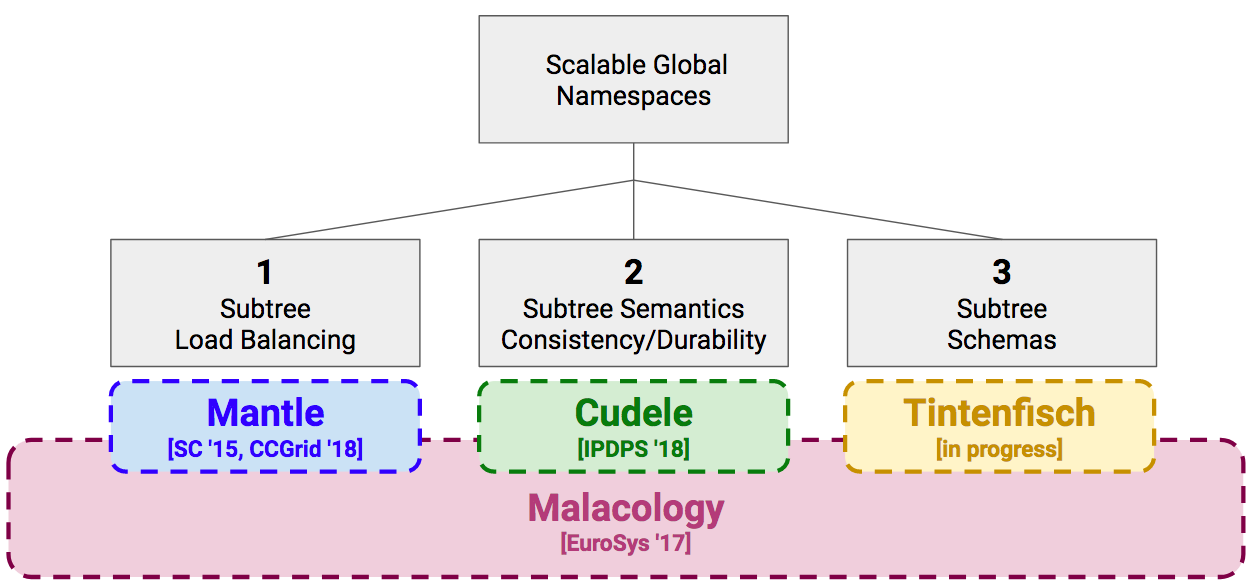
\includegraphics[width=1\textwidth]{./chapters/overview.png}
  \caption{An outline of this thesis.}
  \label{fig:thesis-overview}
\end{figure}

An outline of the thesis is shown in Figure~\ref{fig:thesis-overview}.

Chapter~\ref{chp:related-work} discusses the file system metadata management
problem and shows why today's jobs impose these types of workloads. We also
survey related work for providing scalability while enforcing POSIX IO
semantics. Chapter~\ref{chp:prototyping-platform} describes our prototyping
platform, Ceph, and the interfaces we added to create a programmable storage
system called Malacology.

Chapter~\ref{chp:mantle} describes the Mantle environment and API for load
balancing subtrees across a metadata cluster. We motivate the framework by
measuring the advantages of file system workload locality and examining the
current CephFS implementation designed in~\cite{weil:osdi2006-ceph,
weil:sc2004-dyn-metadata}. We show that the framework can replicate techniques
from related work and show load balancers that work well for different
workloads. Chapter~\ref{chp:mantle-beyond} shows the generality of the approach
by using the Mantle API for load balancing in ZLog, an implementation of the
CORFU~\cite{balakrishnan_corfu_2012} API on Ceph, and for cache management in
ParSplice~\cite{perez:jctc20150parsplice}, a molecular dynamics simulation
developed at Los Alamos National Laboratory.

Chapter~\ref{chp:cudele} describes the Cudele API and framework for relaxing
consistency and durability semantics in a global file system namespace. We
focus on the building blocks called mechanisms and show how administrators can
build application-specific subtrees.  We motivate Cudele by measuring the POSIX
IO overheads using CephFS and by examining current workloads in HPC and
Hadoop/Spark. The microbenchmarks show the performance of individual mechanisms
while the macrobenchmarks model real-world use cases.

Chapter~\ref{chp:tintenfisch} describes Tintenfisch, which lets clients and
servers generate subtrees to reduce network traffic, storage footprints, and
file system metadata load. We examine three motivating examples from three
different domains: high performance computing, high energy physics, and large
scale simulations. We then present namespace schemas for categorizing file
system metadata structure and namespace generators for compacting metadata.

Chapter~\ref{chp:conclusion} concludes and outlines future work.

